% !TeX program = pdflatex
% Alternative (empfohlen, wenn MetaOT genutzt werden soll): xelatex oder lualatex

\documentclass[
amberg, % Titelfolie im CD-Stil (amberg / weiden / amwen / white / orange)
toc=fancy, % toc=normal | fancy | twocolumn | legacy
footlinebox, % Box/Abtrennung in der Fusszeile
notitleshapes, % vermeidet Abhaengigkeit von fehlendem shapes-4.pdf
nometaot % wichtig fuer pdfLaTeX; bei XeLaTeX/LuaLaTeX + installierter MetaOT entfernen
]{OTHAWbeamer}

\usepackage{graphicx}
\usepackage{xcolor}
\usepackage{booktabs}
\usepackage{hyperref}
\usepackage{tikz}
\usetikzlibrary{arrows.meta, positioning}

% ---------------------------
% Meta-Daten
% ---------------------------
\title[Manhattan Buildings]{Visualisierung von Manhattan-Gebaeuden}
\subtitle{Interaktive 3D-Webanwendung mit Filteroptionen und VR-Modus}
\author{Budulak, David \and Renner, Artur}
\institute{OTH Amberg-Weiden}
\date{\today}

% Kontakt-/Abschluss-Frames (Makros kommen aus der Klasse)
\email{david.budulak@oth-aw.de}
\telephone{+49 (0) 17643844150}
\address{Ludwig-Richter-Strasse 7\\92224 Amberg}
\position{EMI / MI / Student}
% optional: Foto fuer contactframe (Pfad relativ zum .tex)
% \photo{images/mein-foto.jpg}

% ---------------------------
% Dokument
% ---------------------------
\begin{document}

    \maketitle

    \begin{frame}{Inhaltsverzeichnis}
        \tableofcontents
    \end{frame}

    % Titelfolie (durch Klasse gestaltet)


    % ---------------------------
    \section{Projektidee}

    \begin{frame}{Projektidee}
        \begin{itemize}
            \item Entwicklung einer interaktiven Visualisierung von Gebaeuden in Manhattan
            \item Gebaeude werden als 3D-Stadtmodell im Browser dargestellt
            \item Nutzerinnen und Nutzer koennen die Ansicht frei erkunden
            \item Filter helfen dabei, bestimmte Gebaeudegruppen sichtbar zu machen
        \end{itemize}

        \vspace{0.5cm}

        \begin{center}
            \Large
            Von Rohdaten zu einer verstaendlichen, begehbaren Stadtansicht
        \end{center}
    \end{frame}

    % ---------------------------
    \section{Funktionen}

    \begin{frame}{Was kann unsere Anwendung?}
        \begin{columns}[T]
            \column{0.48\textwidth}
            \textbf{Interaktive Karte}
            \begin{itemize}
                \item Manhattan als 3D-Ansicht
                \item Zoomen, Drehen und Navigieren
                \item Gebaeude visuell vergleichen
            \end{itemize}

            \vspace{0.3cm}
            \textbf{Filteroptionen}
            \begin{itemize}
                \item Auswahl bestimmter Gebaeudetypen
                \item Einschraenkung nach Eigenschaften
                \item Schnellere Orientierung in grossen Datenmengen
            \end{itemize}

            \column{0.48\textwidth}
            \textbf{Zusatzfunktionen}
            \begin{itemize}
                \item Hervorhebung relevanter Gebaeude
                \item Legende fuer bessere Einordnung
                \item VR-Modus fuer immersives Erkunden
            \end{itemize}

            \vspace{0.3cm}
            \textbf{Ziel}
            \begin{itemize}
                \item Daten nicht nur anzeigen
                \item sondern raeumlich erfahrbar machen
            \end{itemize}
        \end{columns}
    \end{frame}

    % ---------------------------
    \section{Aufbau}

    \begin{frame}{Einfacher Aufbau}
        \begin{center}
            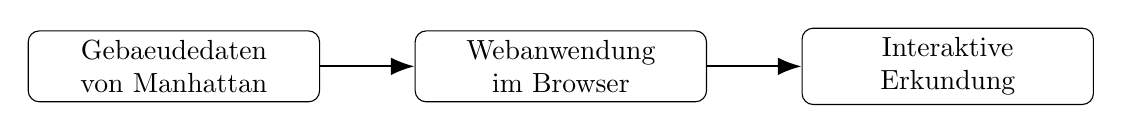
\begin{tikzpicture}[
                node distance=1.2cm,
                box/.style={draw, rounded corners, align=center, minimum width=3.7cm, minimum height=0.9cm},
                arrow/.style={-{Latex[length=3mm]}, thick}
            ]
                \node[box] (data) {Gebaeudedaten\\von Manhattan};
                \node[box, right=of data] (app) {Webanwendung\\im Browser};
                \node[box, right=of app] (user) {Interaktive\\Erkundung};

                \draw[arrow] (data) -- (app);
                \draw[arrow] (app) -- (user);
            \end{tikzpicture}
        \end{center}

        \vspace{0.6cm}

        \begin{itemize}
            \item Die Daten werden in eine 3D-Ansicht uebersetzt
            \item Die Bedienung erfolgt direkt im Browser
            \item Filter und VR-Modus machen die Visualisierung anschaulicher
        \end{itemize}
    \end{frame}

    % ---------------------------
    \section{Live-Demo}

    \begin{frame}{Live-Demo}
        Heute zeigen wir kurz:

        \vspace{0.25cm}

        \begin{enumerate}
            \item Start der Webanwendung
            \item Navigation durch Manhattan
            \item Nutzung der Filteroptionen
            \item Vergleich und Hervorhebung von Gebaeuden
            \item Wechsel in den VR-Modus
        \end{enumerate}

        \vspace{0.7cm}

        \begin{center}
            \Huge Fragen?
        \end{center}
    \end{frame}

\end{document}
